\section{Introduction}

Le projet réalisé dans le cadre de l'enseignement de Conception de Circuits numériques a pour 
objectif de développer des compétences essentielles à la conception de systèmes embarqués, 
notamment la mise au point d'un circuit utilisant un composant logique programmable.
\newline

L'architecture électronique d'un véhicule repose sur une organisation de calculateurs distribués. 
L'exemple retenu s'inspire du fonctionnement d'un calculateur embarqué dans la portière d'une 
automobile, chargé de la gestion des rétroviseurs et des vitres électriques.
\newline

Dans ce contexte, deux sous-ensembles sont distingués : 
\begin{itemize}
    \item un sous-ensemble de supervision, qui génère les commandes pour les moteurs des rétroviseurs et des vitres électriques,
    \item un sous-ensemble d'interface, assurant la communication entre le sous-ensemble de supervision et les autres calculateurs du véhicule.
\end{itemize}

Ce rapport se concentre exclusivement sur ce second sous-ensemble, l'interface microprocesseur, afin d'étudier son rôle et sa conception.

L'un des objectifs principaux est d'appréhender la conception du circuit via la méthode MCSE (Méthode de Conception de Systèmes Électroniques), en mettant l'accent sur les étapes de spécifications et de conception. Le déroulement du rapport suit la logique du diagramme en Y.

\begin{figure}[H]
    \centering
    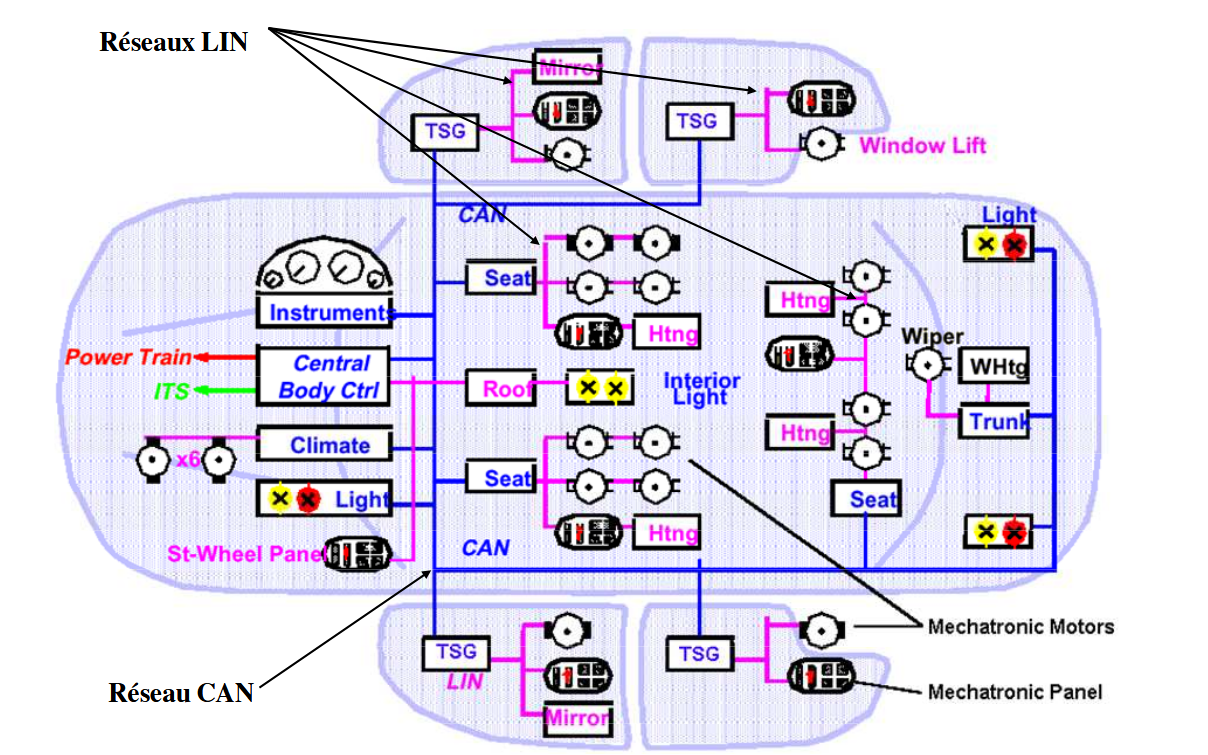
\includegraphics[width=0.8\linewidth]{images/Intro/Architecture_LIN.png}
    \caption{Exemple d'architecture d'un réseau dans un véhicule}
    \label{fig:placeholder}
\end{figure}